\section{System Design} \label{section:design}

The goal of our system is to store the location, and associated information, of a large number of clients who can potentially move around in the real world.
Once the location is stored, our system can serve requests against those clients efficiently, leveraging the physical locality properties.
In this section, we introduce the design, while Section~\ref{section:implementation} discusses some tradeoffs in our implementation.

\subsection{Architecture}

\begin{figure}
\centering
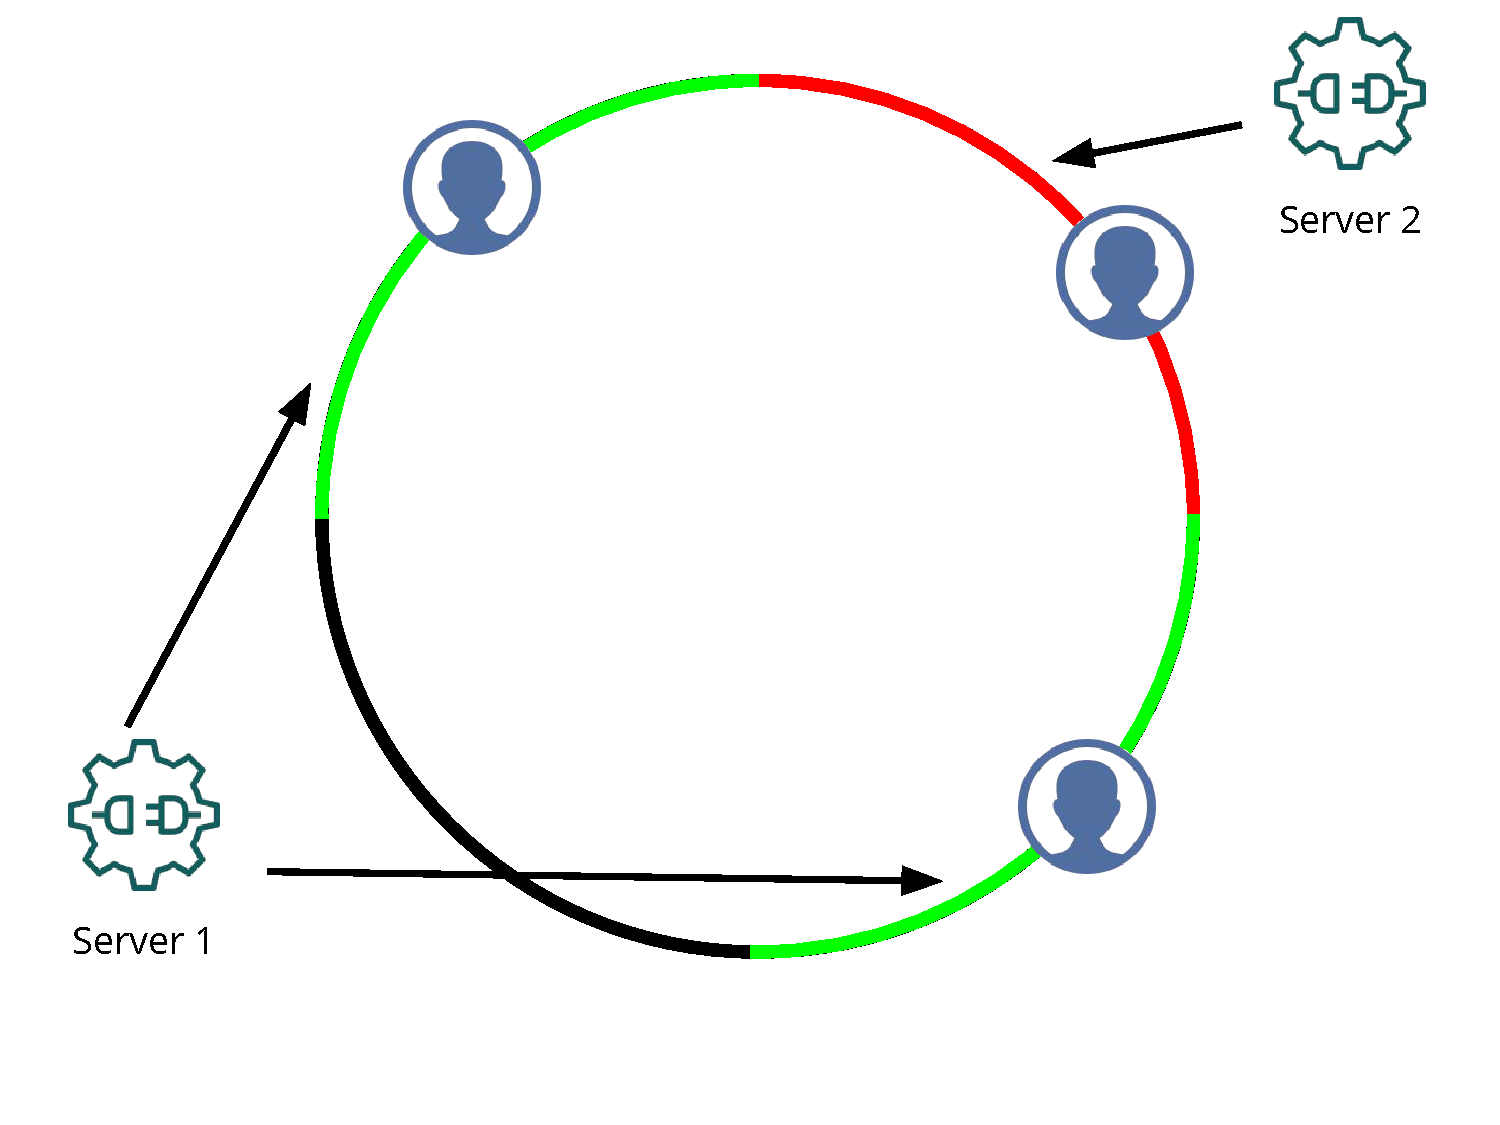
\includegraphics[width=0.6\linewidth]{figures/arch.pdf}
\caption{The Architecture of hDHT.}
\label{fig:arch}
\end{figure}

The architecture of hDHT is shown in Figure~\ref{fig:arch}.
In hDHT, the server control one or more contiguous segments on a \textit{consistent hashing ring}~\cite{}.
Each client has a position in the hashing ring which is determined based on the client physical location, using the \textit{Hilbert curve function}~\cite{}.
Each client thus \textit{registers} with the server that controls the segment containing the client.

In the example, Server 1 controls the two green segments, and stores the data for two clients.
Server 2 controls the red segment, and stores the data only of the client in that segment.
Other servers, not shown, control the rest the DHT curve.

\subsection{Client Interface}

Clients of hDHT are likely to be on a mobile device, as they should follow and record precisely the location of the user.
Servers cannot perform RPCs towards the clients, because the clients might be behind a restrictive firewall.
For this reason, our design moves most of the computation and networking to the server, and initiates all client-server communication from the client.

Each client is identified by a 160-bit node identifier.
This identifier is opaque to the client.
The client additionally stores its own position, as obtained from the GPS senstor, and the address of the server it is registered with.
The client interacts primarily with the registering server, but any time it can retrieve the address of the server responsible for any point in the curve.

Servers store simple client metadata, in the form of string key-value pairs.
Each server serves metadata requests only for the clients it is responsible for, which ensures consistency.

The full client-server interface is shown in Figure~\ref{fig:client-server}.

\begin{figure}
\small
\begin{itemize}
\item $\textsc{FindControllingServer}(\textit{node\_id}) \rightarrow \textit{address}$: find the address of the server controlling the given node ID; this request succeeds even if the node ID does not correspond to any client registered with the server
\item $\textsc{FindServerForPoint}(\textit{position}) \rightarrow \textit{address}$: find the address of the server controlling the given position
\item $\textsc{ClientHello}(\textit{position}, \textit{node\_id}) \rightarrow \textit{ok}, \textit{node\_id}$: register the client against this server; the client transmits both its own position and the previously obtained node ID, if available; the server responds \textit{Created} if the client was newly registered, \textit{AlreadyExists} if it recognized the previous node ID, or \textit{WrongServer} if the server is not responsible for the region of the Hilbert curve corresponding to \textit{position}.
\item $\textsc{Move}(\textit{position}) \rightarrow \textit{ok}, \textit{node\_id}, \textit{address}$: informs the server that the client moved; the server replies with the new node ID for the client, and either \textit{SameServer} or \textit{DifferentServer}, to indicate what server is now responsible for the client; if the client receives \textit{DifferentServer}, it must register with the new server
\item $\textsc{SetMetadata}(\textit{key}, \textit{value})$: set metadata for the calling client
\item $\textsc{GetMetadata}(\textit{node\_id}, \textit{key}) \rightarrow \textit{value}$: get metadata about the given client; the server forwards the request to the controlling server if needed
\end{itemize}
\caption{The hDHT client-server protocol}
\label{fig:client-server}
\end{figure}

\subsection{Hilbert Curves}

Client node IDs define the position of a client in the consistent hashing ring.
To facilitate location based queries, the node IDs are generated using a \textit{locality sensitive hash} that uses a Hilbert curve.

A Hilbert curve, or \textit{space-filling curve}, is a curve that passes all points in a grid exactly once and does not self intersect.
Hilbert curve can be constructed for grids of arbitrary dimension.
The Hilbert curve of order $k$, which covers the grid of size $2^k \times 2^k$, is constructed as a fractal, by refining the Hilbert curve of order $k-1$.
An efficient $O(k)$ algorithm exists to convert any point to the Hilbert curve to its coordinates in the grid and viceversa.

\subsection{Mapping Hilbert Curves to Consistent Hashing}

hDHT uses the Hilbert curve concept to generate the ID of the client.
First, the physical position of the client is mapped to a point in a rectangular Earth-sized grid.
Then, the point in the grid is converted to a point in the Hilbert curve, which provides the high bits of the node IDs.
The remaining low bits are assigned randomly.
This is a locality sensitive hashing because clients who are phyisically close will have similar Hilbert curve values, and thus will share some of the high bits of their node IDs.
Additionally, clients with similar high bits in the node IDs are more likely to be assigned to the same server, which improves the efficiency of serving requests.

Furthermore, hDHT must partition the grid in a way that each server controls a rectangular region.
This way, search requests can be served efficiently by dividing the query into disjoint rectangles.
To do so, the Hilbert curve must be partitioned into \textit{intervals} of the form:
\begin{align}
\left[k 2^i, (k+1) 2^i\right)
\end{align}
(with $k$, $i$ integers, and $i$ less than the order of the curve).
Intervals of this form can be shown to be non-overlapping in the grid.

Each server controls one or more of these intervals.
The server has complete information over the intervals it controls, and relies on other servers for the rest of the grid.


\subsection{Search Inside a Single Interval}
For each controlled interval of the Hilbert curve, the server maintains an \textit{Hilbert RTree}~\cite{} of the clients.
This is a data structure that allows efficient insertion, deletion and query by rectangle.

FINISHME...

\subsection{Search Across the Whole Space}
To perform a search, the server needs to efficiently identify which intervals of the DHT are partially covered by the search rectangle, and then perform the search within the interval.

The takes advantage of an important property of Hilbert curves: if a point is outside a rectangle in the Hilbert curve, all points on the curve between that point and the next rectangle corner are also outside the corner.

The server then uses the following algorithm:
\begin{enumerate}
\item First it computes the Hilbert values $h_0, h_1, h_2, h_3$ of the four corners of the rectangle, where $h_0$ is the smallest Hilbert value and $h_3$ is the largest
\item The algorithm keeps track of a \textit{current point}, initialized to $h_0$.
\item Then, it checks if the current point is inside the query rectangle.
\item If so, it finds the interval that contains the current point from the DHT
\item For a local interval, it uses the RTree to perform the search
\item For a remote interval, it forwards the search to the server that controls the interval, and merges the result
\item The algorithm then proceeds at point $h'$ immediately after the end of the interval in the Hilbert curve $h' = (k+1) 2^i$
\item If the current point is outside the query rectangle, the algorithm sets to current point to the minimum of $h_i$ that is strictly greater than the current point (in other words, it skips to the next corner of the query rectangle in the Hilbert curve).
\item The algorithm terminates when the current point is greater than $h_3$.
\end{enumerate}

\subsection{Routing and Load Balancing}

To make it possible for servers to join and leave the DHT easily, each server does not keep precise information on which intervals are owned by whom.

At initialization time, the server starts with a single peer, which it assumes controls the whole table.
The server registers with this initial peer, who responds with a list of interval it knows about.
The server then registers with each of the newly discovered peers, which will further send more and more precise information.

Additionally, when a new server joins the DHT, each peers that learns about the new server performs load balancing on the portion of the table it controls, by spilling the intervals it controls and transferring control of the newly created subintervals to the new server.
Intervals must be split in half at each step, because they must be power-of-2 sized to be rectangular in the grid.

An interval will be considered for splitting if it is larger than a threshold (in logarithmic size), or if the number of clients exceeds a threshold.
In the former case, the interval is split in half only once, and one half is sent to the new server.
In the latter case, the newly created half interval with the most clients is split again until the number of clients is below the threshold.
Then, the half interval with the least clients is sent to the new server.

Servers automatically move the metadata and client IDs during DHT rebalancing, but they do not inform clients.
Clients learn of the rebalancing by receiving a redirection error the next time they attempt to perform a request.
